
\documentclass[a4paper, 12pt]{book}
%\usepackage[T1]{fontenc}

\usepackage[a4paper, left=2.5cm, right=2.5cm, top=3cm, bottom=3cm]{geometry}
\usepackage{times}
\usepackage[utf8]{inputenc}
\usepackage[spanish]{babel} % Comenta esta línea si tu memoria es en inglés
\usepackage{url}
%\usepackage[dvipdfm]{graphicx}
\usepackage{graphicx}
\usepackage{float}  %% H para posicionar figuras
\usepackage[nottoc, notlot, notlof, notindex]{tocbibind} %% Opciones de índice
\usepackage{latexsym}  %% Logo LaTeX
\usepackage{float}
\usepackage{listings}
\usepackage{xcolor}

\lstset{
  basicstyle=\ttfamily\footnotesize,
  breaklines=true,
  backgroundcolor=\color{gray!10},
  frame=single,
  captionpos=b
}


% Escribe el título y el nombre del autor / autora para que se use bien
% en otras partes de la plantilla
% Dependiendo de las partes de la plantilla, a veces aparecerán tal
% cual los escribas, a veces totalmente en mayúsculas, a veces de otras
% formas
\title{Edición de Escenas 3D mediante Voz}
\author{Pablo Esteban Camuendo Carlosama}

% Guarda el título, el autor y la fecha en variables
\makeatletter
\let\thetitle\@title
\let\theauthor\@author
\let\thedate\@date
\let\cleardoublepage\clearpage
\makeatother

\renewcommand{\baselinestretch}{1.5}  %% Interlineado

\begin{document}

\renewcommand{\refname}{Bibliografía}  %% Renombrando
\renewcommand{\appendixname}{Apéndice}


%%%%%%%%%%%%%%%%%%%%%%%%%%%%%%%%%%%%%%%%%%%%%%%%%%%%%%%%%%%%%%%%%%%%%%%%%%%%%%%%
% PORTADA

\begin{titlepage}
\begin{center}

\includegraphics[scale=0.6]{img/URJ_logo_Color_POS.png}

\vspace{1.75cm}

\LARGE
ESCUELA DE INGENIERÍA DE FUENLABRADA
\vspace{1cm}

\LARGE
INGENIERÍA EN SISTEMAS AUDIOVISUALES Y MULTIMEDIA

\vspace{1cm}
\LARGE
\textbf{TRABAJO FIN DE GRADO/MÁSTER}

\vspace{2cm}

\Large
\MakeUppercase{\thetitle}

\vspace{2cm}

\large
Autor : \theauthor \\
Tutor : Dr. Jesús María González Barahona\\
Cotutor: (si procede)
\vspace{1cm}

\large
Curso académico 2024/2025

\end{center}
\end{titlepage}

\newpage
\mbox{}
\thispagestyle{empty} % para que no se numere esta pagina



%%%%%%%%%%%%%%%%%%%%%%%%%%%%%%%%%%%%%%%%%%%%%%%%%%%%%%%%%%%%%%%%%%%%%%%%%%%%%%%%
%%%% Licencia
\clearpage
\pagenumbering{gobble}
\chapter*{}

\vspace{12cm}

%% Licencia de publicación en abierto elegida
%% Ver detalles en https://ofilibre.urjc.es/guias/tfg-abierto/

\begin{flushright}
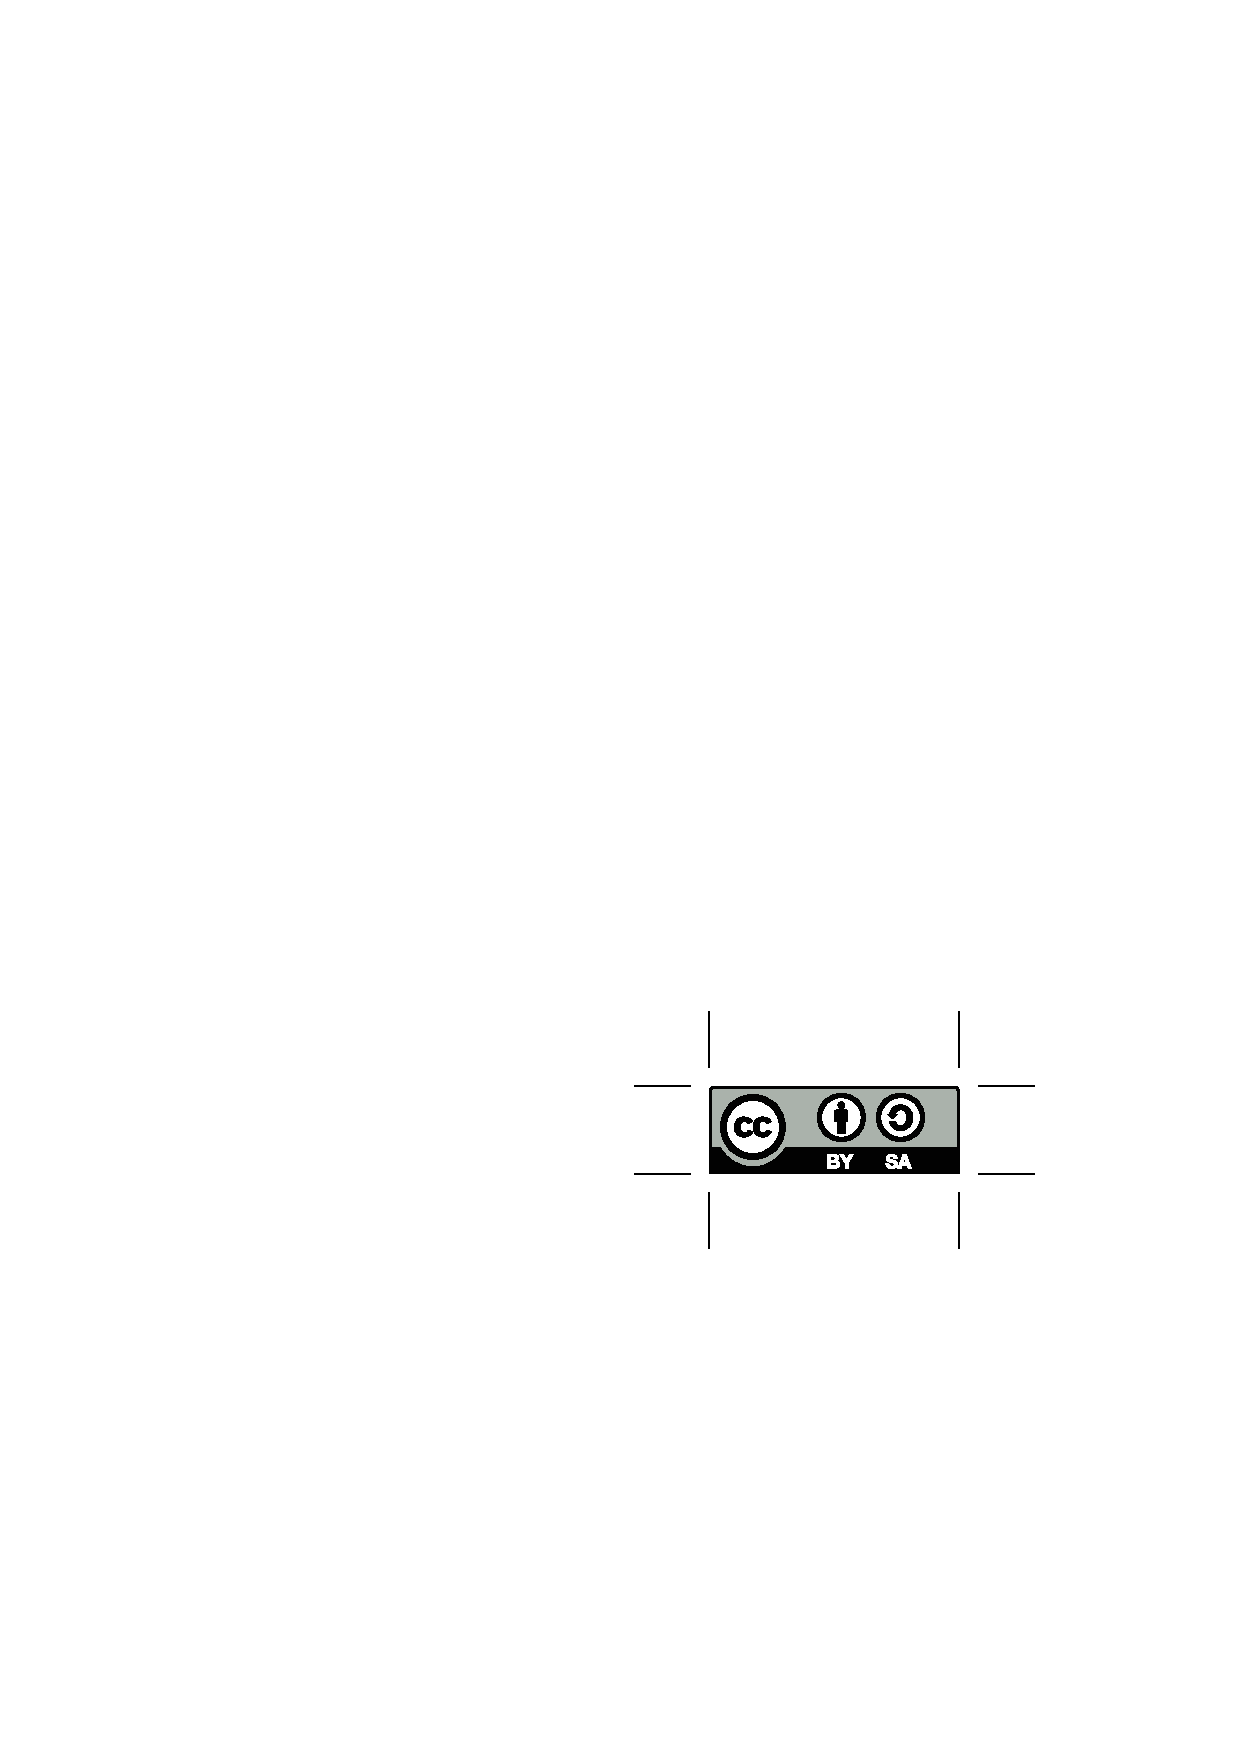
\includegraphics[scale=0.6]{img/by-sa}
%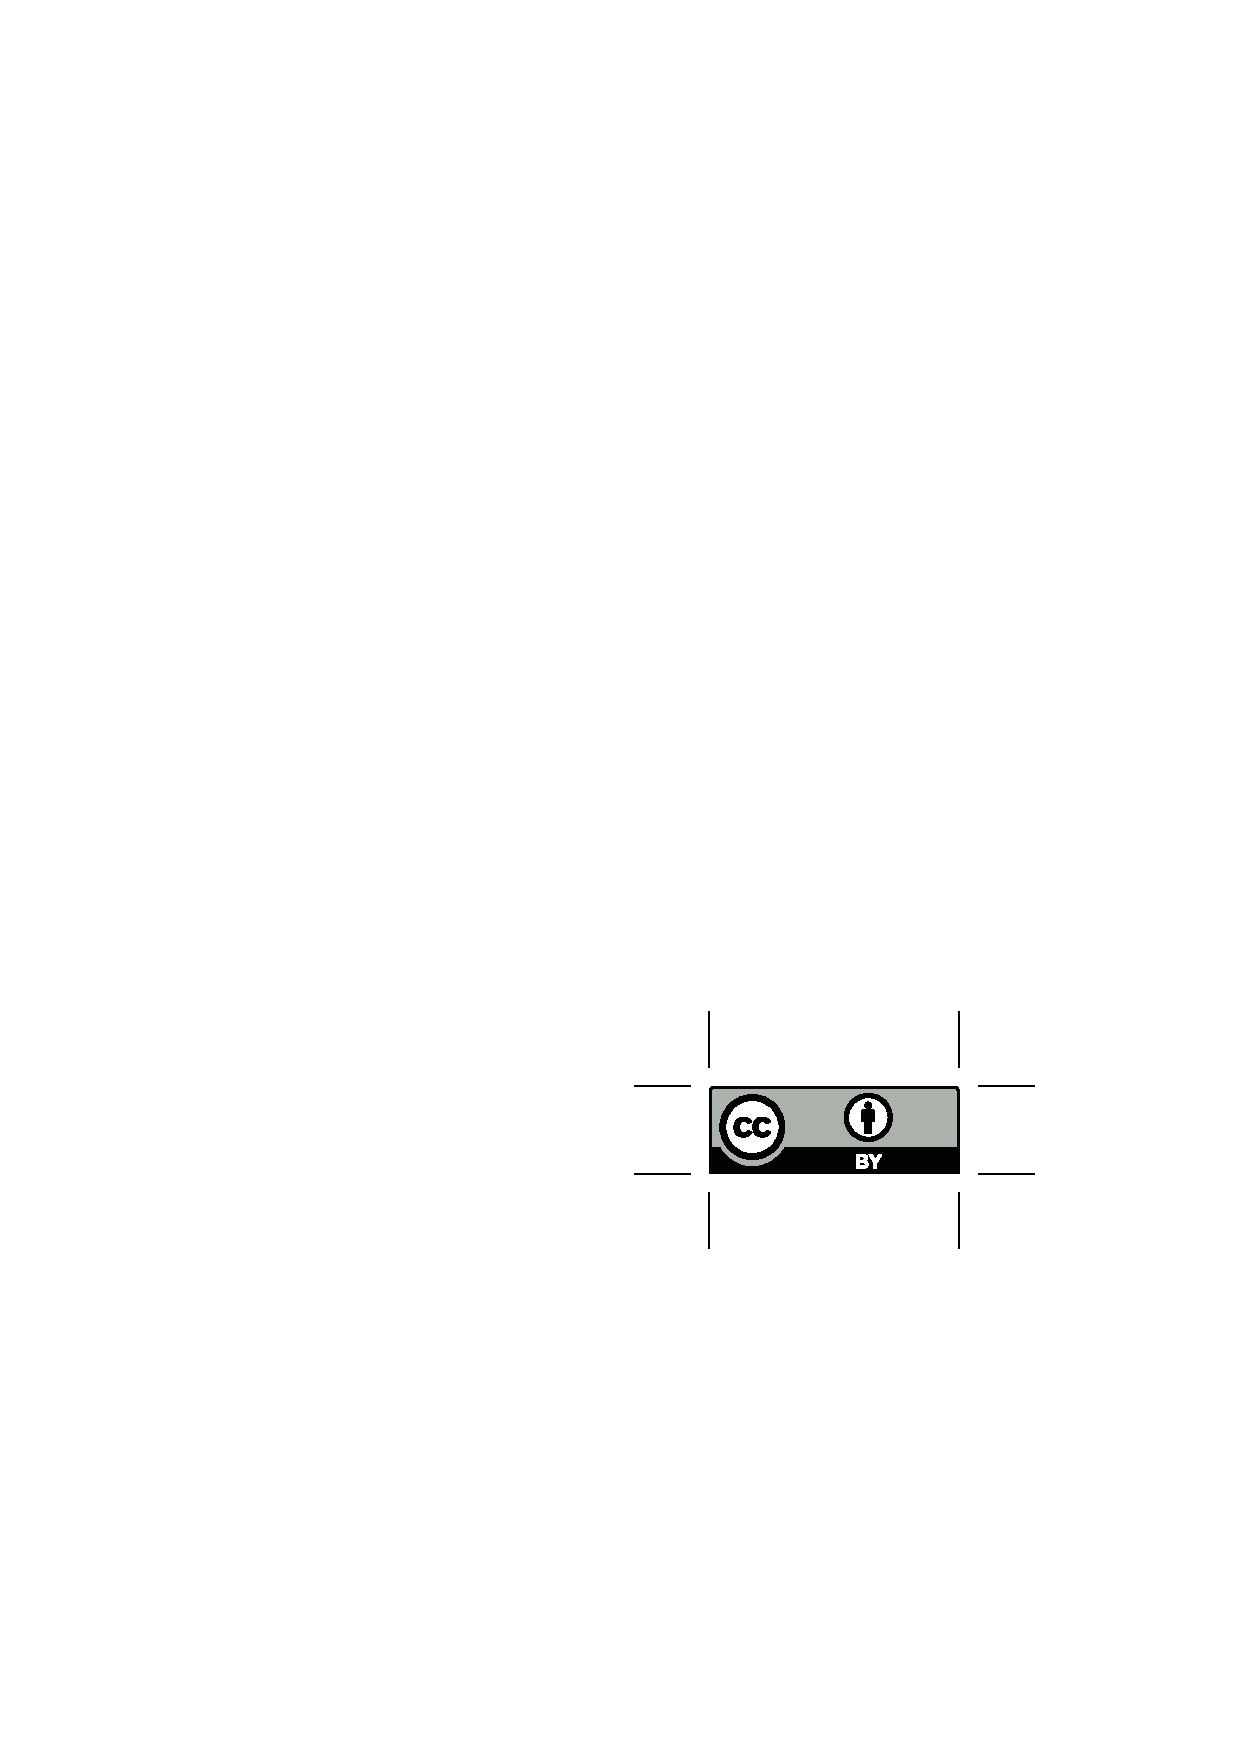
\includegraphics[scale=0.6]{img/by}

%% Poner el año adecuado
\noindent©2025 \theauthor  \\
Algunos derechos reservados  \\
Este documento se distribuye bajo la licencia \\
``Atribución-CompartirIgual 4.0 Internacional'' de Creative Commons, \\
disponible en \\
\url{https://creativecommons.org/licenses/by-sa/4.0/deed.es}
\end{flushright}

%%%%%%%%%%%%%%%%%%%%%%%%%%%%%%%%%%%%%%%%%%%%%%%%%%%%%%%%%%%%%%%%%%%%%%%%%%%%%%%%
%%%% Dedicatoria

\chapter*{}
\pagenumbering{Roman} % para comenzar la numeracion de paginas en numeros romanos
\begin{flushright}
\textit{Dedicado a \\
mi familia.}
\end{flushright}

%%%%%%%%%%%%%%%%%%%%%%%%%%%%%%%%%%%%%%%%%%%%%%%%%%%%%%%%%%%%%%%%%%%%%%%%%%%%%%%%
%%%% Agradecimientos

\chapter*{Agradecimientos}
%\addcontentsline{toc}{chapter}{Agradecimientos} % si queremos que aparezca en el índice
\markboth{AGRADECIMIENTOS}{AGRADECIMIENTOS} % encabezado 

Quisiera expresar mi más sincero agradecimiento a todas las personas e instituciones que han hecho posible la realización de esta tesis de grado:

En primer lugar, mi familia, durante todos estos años de estudio, por su apoyo incondicional y esfuerzo, su comprensión y aliento continuo. Su fe en mí es la mayor inspiración. Ellos siempre han dicho que la educación es la base de todo lo que puedo construir a continuación y es gracias a ellos que he podido llegar aqui. Gracias, mamá y papá

A mi hermana, que a sido un constante apoyo y de la cual quiero ser un ejemplo a seguir, que sepa que el desarollo de uno mismo es difícil, pero satisfactorio al final.

A mi tutor de tesis, por su guía, paciencia y conocimientos compartidos a lo largo de este proceso. Su experiencia ha sido crucial para el desarrollo de este trabajo.

Finalmente, a todos aquellos que de una u otra manera han contribuido a mi crecimiento personal y profesional durante mi etapa universitaria.

A todos, mi más profunda gratitud.


%%%%%%%%%%%%%%%%%%%%%%%%%%%%%%%%%%%%%%%%%%%%%%%%%%%%%%%%%%%%%%%%%%%%%%%%%%%%%%%%
%%%% Resumen

\chapter*{Resumen}
%\addcontentsline{toc}{chapter}{Resumen} % si queremos que aparezca en el índice
\markboth{RESUMEN}{RESUMEN} % encabezado

RESUMEN LO HAGO AL FINAL ....



%%%%%%%%%%%%%%%%%%%%%%%%%%%%%%%%%%%%%%%%%%%%%%%%%%%%%%%%%%%%%%%%%%%%%%%%%%%%%%%%
%%%% Resumen en inglés

\chapter*{Summary}
%\addcontentsline{toc}{chapter}{Summary} % si queremos que aparezca en el índice
\markboth{SUMMARY}{SUMMARY} % encabezado

Here comes a translation of the ``Resumen'' into English. 
Please, double check it for correct grammar and spelling.
As it is the translation of the ``Resumen'', which is supposed to be written at the end, this as well should be filled out just before submitting.


%%%%%%%%%%%%%%%%%%%%%%%%%%%%%%%%%%%%%%%%%%%%%%%%%%%%%%%%%%%%%%%%%%%%%%%%%%%%%%%%
%%%%%%%%%%%%%%%%%%%%%%%%%%%%%%%%%%%%%%%%%%%%%%%%%%%%%%%%%%%%%%%%%%%%%%%%%%%%%%%%
% ÍNDICES %
%%%%%%%%%%%%%%%%%%%%%%%%%%%%%%%%%%%%%%%%%%%%%%%%%%%%%%%%%%%%%%%%%%%%%%%%%%%%%%%%

% Las buenas noticias es que los índices se generan automáticamente.
% Lo único que tienes que hacer es elegir cuáles quieren que se generen,
% y comentar/descomentar esa instrucción de LaTeX.

%%%% Índice de contenidos
\tableofcontents 
%%%% Índice de figuras
\cleardoublepage
%\addcontentsline{toc}{chapter}{Lista de figuras} % para que aparezca en el indice de contenidos
\listoffigures % indice de figuras
%%%% Índice de tablas
%\cleardoublepage
%\addcontentsline{toc}{chapter}{Lista de tablas} % para que aparezca en el indice de contenidos
%\listoftables % indice de tablas


%%%%%%%%%%%%%%%%%%%%%%%%%%%%%%%%%%%%%%%%%%%%%%%%%%%%%%%%%%%%%%%%%%%%%%%%%%%%%%%%
%%%%%%%%%%%%%%%%%%%%%%%%%%%%%%%%%%%%%%%%%%%%%%%%%%%%%%%%%%%%%%%%%%%%%%%%%%%%%%%%
% INTRODUCCIÓN %
%%%%%%%%%%%%%%%%%%%%%%%%%%%%%%%%%%%%%%%%%%%%%%%%%%%%%%%%%%%%%%%%%%%%%%%%%%%%%%%%

\cleardoublepage
\chapter{Introducción}
\label{sec:intro} % etiqueta para poder referenciar luego en el texto con ~\ref{sec:intro}
\pagenumbering{arabic} % para empezar la numeración de página con números
***INTRODUCCION GENERICA.***

Con el gran avance en tecnologias, la realidad virtual (VR) ha experimentado un gran crecimiento en los ultimos años, gracias a la evolución de tecnologías web accesibles y de código abierto. A-Frame es un framework de las tecnologias antes mencionadas, basado en WebXR y Three.js, permite la creacion y configuración de escenas aprovechando directamente el navegador usando HTML y JavaScript.

Unido a este framework tendremos el desarollo del reconocimiento del habla que permitira controlar la escena mediante comandos de voz.  La combinación de ambas tecnologías ofrece un enfoque innovador para mejorar la accesibilidad, la usabilidad y la inmersión en aplicaciones de realidad virtual dejando de lado los medios tradicionales.

En este Trabajo Fin de Grado se muestra el desarollo de una aplicacion para la creacion y edicion de escenas en 3D, en donde el usuario puede interactuar con objetos en la escena para editar algunos de sus parametros o incluso crear objetos de una libreria, todo ello mediante comandos de voz. De tal manera que se facilitara la interraccion con la escena de forma dinamica, pudiendo observar los cambios realizados al momento.

**************************************************

En este capítulo se introduce el proyecto.
Debería tener información general sobre el mismo, dando la información sobre el contexto en el que se ha desarrollado.

contextualizar el estado de la aplicacion ... y de donde salio...

********************

La realidad virtual (VR) ha dado un gran paso en la ultima decada, haciendo que el uso de tecnologias web y aplicaciones de codigo libre este al alcance de todos, lo que ha creado muchas oportunidades de desarollo de diferentes aplicaciones que permiten ver y crear escenas en 3D.

Centrandonos en el desarollo de aplicaciones para entornos como el navegador(browser) debemos tener en cuenta que se desarollan bajo la construccion de WebXR, al rededor de 2010 se inicio con el desarollo de three.js una biblioteca para crear graficos en 3D, este desarollo junto a el lanzamiento de WebGL en el 2011 permitio el uso de graficos en 3D en los navegadores. Tras esto se desarollo un predecesor de WebXR llamado WebVR, esta fue una API creada por Mozilla en el 2014 para acceder a dispositivos de realidad virtual por medio de navegadores, aunque existian limitaciones al no soportar la realidad aumentada, hoy en dia WebXR unifica la VR y la AR mejoranto compatibilidad y rendimiento, adaptandose a deferentes navegadores ademas de Mozilla.

Con este desarollo se han permitido las experiencias inmersivas mediante dispositivos externos como las gafas AR/VR.

**************************
\section{Estructura de la memoria}
\label{sec:estructura}

El resto de la memoria se estructurara de la siguiente manera:

\begin{itemize}
    \item ~\ref{chap:Tecnologías utilizadas} Tecnologías utilizadas: Se muestran todas las tecnologías utilizadas durante el desarrollo del proyecto, desde las principales como A-Frame para la construcción de entornos inmersivos en el navegador, hasta herramientas auxiliares como Node.js o WebXR. Se da una breve descripción de cada tecnología, el contexto de uso y su papel dentro de cada una de las demos.
  
    \item ~\ref{chap:Desarollo} Desarollo del Proyecto: Se detalla el proceso completo de creación donde se implementaron dos versiones de la demo: una que usa la Web Speech API directamente en el navegador, y otra que envía audio a un servidor local para procesarlo con AssemblyAI.
  
    \item ~\ref{chap:descripcion} Descripcion del resultado:
   Aquí se muestra el resultado final de ambas demos:

Descripción para el usuario: Se explica qué funcionalidades incluye cada demo, cómo se activan los comandos por voz y cómo se muestra la transcripción dentro del entorno 3D.

Descripción del comportamiento de la interfaz: Se detalla cómo se representa la transcripción en la escena VR/AR, así como la lógica de actualización dinámica de textos en el espacio virtual.
  
    \item ~\ref{chap:experimentos} Experimentos y validacion 
    \item ~\ref{chap:resultados}  Resultados
    \item ~\ref{chap:conclusiones} Conclusiones 
    \item Manual de Uso ~\ref{app:manual}
\end{itemize}


%%%%%%%%%%%%%%%%%%%%%%%%%%%%%%%%%%%%%%%%%%%%%%%%%%%%%%%%%%%%%%%%%%%%%%%%%%%%%%%%
% OBJETIVOS %
%%%%%%%%%%%%%%%%%%%%%%%%%%%%%%%%%%%%%%%%%%%%%%%%%%%%%%%%%%%%%%%%%%%%%%%%%%%%%%%%
\section{Objetivo general} % título de sección (se muestra)
\label{sec:objetivo-general} % identificador de sección (no se muestra, es para poder referenciarla)

El trabajo de fin de grado consiste en la creacion de un componente dedicado para A-Frame que se pueda usar para reconocimiento de voz en comandos para crear y editar escenas en 3D, todo ello usando navegadores compatibles.


\section{Objetivos específicos}
\label{sec:objetivos-especificos}

Los objetivos específicos se pueden entender como las tareas en las que se ha desglosado el objetivo general.
Y, sí, también vienen en infinitivo.
\begin{itemize}
\item Investigacion del uso de aplicaciones para reconocimiento de voz (Speech to Text).
\item Implementar escena simple con A-Frame para lectura de un texto y plasmarlo en un panel de A-Frame.
\item Desarrollar una escena que permita reconocer la voz y se imprima la trascripcion en un panel de A-Frame
\item Creacion de comandos de voz obtenidos de la transcripcion del "Speech to Text".
\item Creacion de componentes separados para Crear, Editar, Eliminar, Ayuda.
\item Investigacion de reconocieminto de voz para gafas de VR/AR.
\item Creacion de un servidor privado para el uso de gafas VR/AR
\item Compatibilidad de codigo con demos para escritorio y gafas VR/AR.
\end{itemize}

%%%%%%%%%%%%%%%%%%%%%%%%%%%%%%%%%%%%%%%%%%%%%%%%%%%%%%%%%%%%%%%%%%%%%%%%%%%%%%%%
%%%%%%%%%%%%%%%%%%%%%%%%%%%%%%%%%%%%%%%%%%%%%%%%%%%%%%%%%%%%%%%%%%%%%%%%%%%%%%%%
% ESTADO DEL ARTE %
%%%%%%%%%%%%%%%%%%%%%%%%%%%%%%%%%%%%%%%%%%%%%%%%%%%%%%%%%%%%%%%%%%%%%%%%%%%%%%%%

\cleardoublepage
\cleardoublepage % empezamos en página impar

\chapter{Tecnologías utilizadas}
\label{chap:Tecnologías utilizadas}

El proyecto, utiliza la interfaz webkitSpeechRecognition para implementar el reconocimiento de voz en el navegador. Esta interfaz es una versión específica para WebKit de la API de reconocimiento de voz de la Web Speech API, que permite a las aplicaciones web convertir el habla en texto.

Además, el proyecto emplea tecnologías web estándar como HTML, CSS y JavaScript para construir la interfaz de usuario y manejar la lógica del cliente. Estas tecnologías trabajan conjuntamente para proporcionar una experiencia interactiva de reconocimiento de voz directamente en el navegador.

Se creo un flujo de trabajo extra para el uso del proyecto en gafas de VR/AR, debido a la creacion de un servidor privado lanzado con Node.js → Para ejecutar el servidor backend. framework HTTP → Para manejar las solicitudes del cliente. AssemblyAI API → Servicio externo de reconocimiento de voz. Fetch → Para enviar los datos de audio a AssemblyAI desde el servidor.

** PONER ALGUNA CITA EN CADA APARTADO
SPEECH 
    ** W3C
CONSTRUCCION SOBRE LOS OBJETOS
A-FRAME > THREE > WEBXR > WEBGL
A FRAME HABLAR DE COMPONENTES, CAPTURAS, ACCIONES, LLAMADOS, CODIGO, ESCENA

HABLAR CON MAS IMPORTANCIA Y EXTENSION 


\section{Tecnologias de reconocimiento de voz} 
\label{sec:seccion1}

El reconocimiento de voz en navegadores permite a los usuarios interactuar con aplicaciones web y contenido utilizando su voz en lugar de escribir. Esto abre un mundo  de posibilidades para la accesibilidad, la productividad y la creación de experiencias de usuario más interactivas.

\subsection{Whisper}

En primera instancia se planeaba trabajar con Whisper, un modelo de "Speech Recognition" de OpenAI que se destaca por su capacidad para transcribir audio en múltiples idiomas con alta precisión, incluso en condiciones de ruido o con variaciones en el acento del hablante, con el objetivo de integrarlo al proyecto.

Whisper\footnote{Whisper OpenAI github  ~\cite{whisper}.} jugaba una parte esencial. se eligio como primera opcion debido a la arquitectura robusta y de codigo libre, como parte de la investigación, se analizaron los requisitos técnicos para la implementación, incluyendo dependencias, consumo de recursos, y compatibilidad con otros componentes del sistema.

\begin{figure}[H]
    \centering
    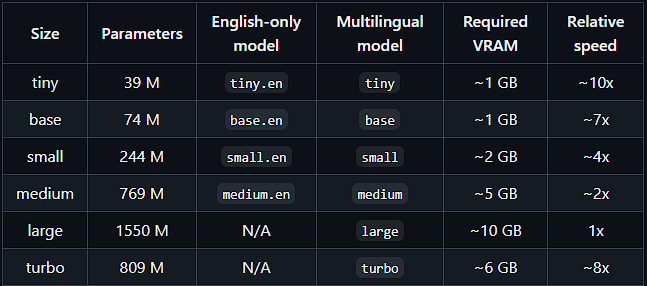
\includegraphics[width=0.8\linewidth]{img/Whisper_github.png}
    \caption{Modelos de Whisper}
    \label{fig:models-Whisper}
\end{figure}

Whisper presenta los modelos que se pueden ver en la Figura~\ref{fig:models-Whisper}. Se pueden observar diferentes tamaños de modelos, cada uno con distintos niveles de precisión, velocidad y requerimientos de hardware.

Los modelos mas grandes (medium,large)son altamente demandantes de GPU, esto hace que los modelos tengas mucha mas precision pero que su velocidad sea mas afectada. Para menor latencia los modelos mas pequeños (tiny, base, small) son mejores, ya que su demanda de hardware es menor.

Alguno de los problemas que presento whisper fue el tamaño de los modelos, ya que incluso el modelo más pequeño (tiny) pesa varios cientos de MB.Se necesita PyTorch y dependencias que no están disponibles en entornos web estándar (como JS/WebAssembly). Ademas del uso intensivo de GPU/CPU, lo cual no es viable en la mayoría de navegadores móviles o de escritorio.

\subsection{Whisper Web}

Actualmente algunos proyectos han empezado a portar versiones ligeras al navegador (construcciones en WebAssembly o ONNX). Un ejemplo de esto es Whisper Web\footnote{Whisper Web Hugging Face  ~\cite{whisperweb}.}

\begin{figure}[H]
    \centering
    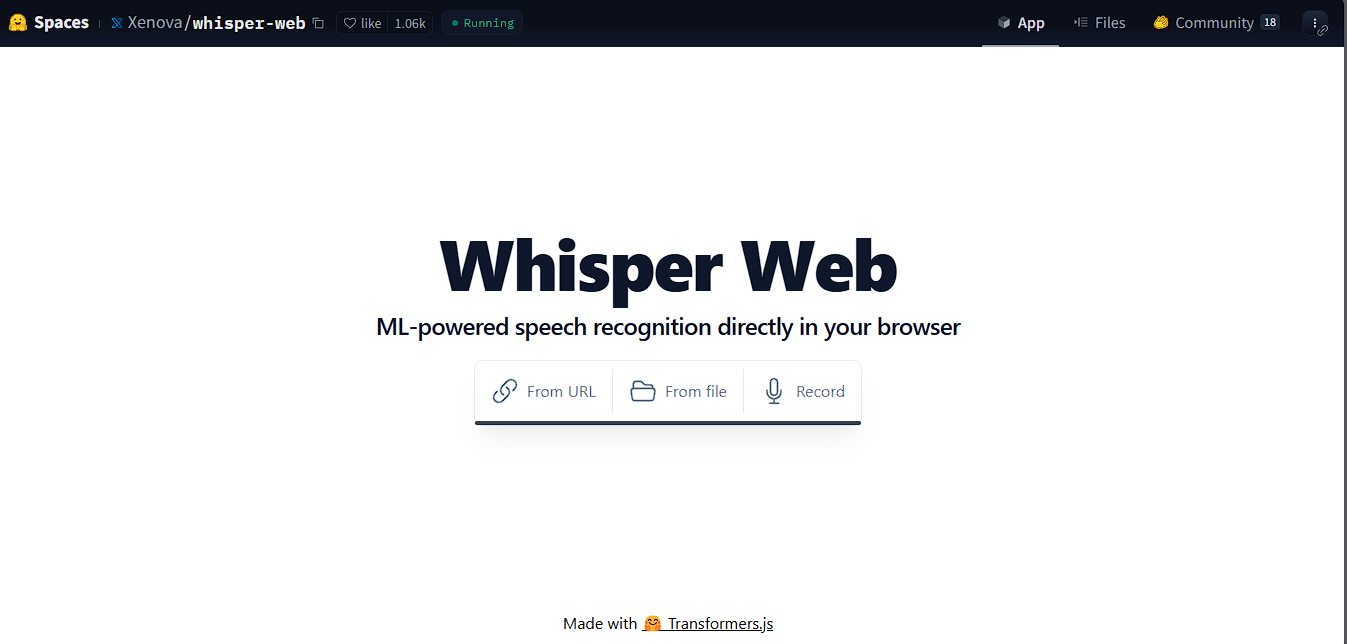
\includegraphics[width=0.8\linewidth]{img/WhisperWeb.png}
    \caption{Whisper Web}
    \label{fig:WhisperWeb}
\end{figure}

En la Figura~\ref{fig:WhisperWeb} se muestra un proyecto de la comunidad que busca llevar Whisper al navegador, sin la necesidad de un back-end. Para ello se usan tecnologias como:
\begin{itemize}
    \item WebAssembly (WASM): para correr código pesado directamente en el navegador.
    \item ONNX (Open Neural Network Exchange): para convertir modelos de PyTorch a un formato más portable.
    \item WebGPU o WebGL: para aprovechar el hardware del usuario (si es compatible).
\end{itemize}

Para ello se da uso a la plataforma y comunidad de Huggind Face enfocada en el desarrollo, distribución y uso de modelos de inteligencia artificial. 

El funcionamiento en esta aplicacion web es el siguiente: 
\begin{itemize}

    \item 1- Se carga un archivo de audio o se graba la voz.
    \item 2- En el navegador elige una versión comprimida del modelo Whisper y la eleccion del lenguaje si el usuario lo desea.
    \item 3- El modelo se ejecuta localmente en el navegador (no sube tu audio a la nube).
    \item 4- La app procesa el audio y muestra la transcripción en pantalla.
    \item 5- El navegador puede exportar la informacion.
\end{itemize}
Esta idea se descarto debido a la complejidad de implementacion en el navegador, ya que ejecutar modelos de reconocimiento de voz como Whisper directamente en la web implica múltiples desafíos técnicos. Entre ellos destacan el alto consumo de recursos, la falta de soporte en entornos como WebAssembly/WebGPU, y la necesidad de trasncribir y optimizar los modelos para que puedan ejecutarse localmente en el cliente sin afectar la experiencia del usuario.

Además, el peso de los modelos de en sus versiones más pequeñas, puede afectar significativamente los tiempos de carga y procesamiento, especialmente en dispositivos móviles o con hardware limitado. Por estas razones, se optó por explorar soluciones alternativas que pudieran integrarse de manera más eficiente dentro del  del proyecto.


\subsection{Web Speech API}

La principal tecnología nativa para reconocimiento de voz directamente en los navegadores es la Web Speech API, específicamente su interfaz SpeechRecognition.

La Web Speech API fue introducida como un borrador por el W3C (World Wide Web Consortium) en 2012. Aunque algunas partes de la API, como la síntesis de voz (SpeechSynthesis), han alcanzado un estado de recomendación, la parte de reconocimiento de voz (SpeechRecognition) aún se considera un borrador de trabajo. Sin embargo, ha sido implementada en la mayoría de los navegadores modernos, aunque con diferentes niveles de soporte y posibles requisitos de prefijos específicos del navegador (ej: webkitSpeechRecognition en Chrome), por ejemplo el uso de esta API en navegadores especificos para gafas VR/AR como las quest3 es directamente imposible, debido a que no hay soporte para ello, por esto lo mas factible para el uso de reconocimiento de voz en casos como estos es usar un back-end que reciba las peticiones y chucks de audio del cliente y esta mismo las transcriba devolviendo asi el texto transcrito.

El uso principal que le dariamos para este proyecto sera el "SpeechRecognition" para convertir la voz en texto. Es cierto que la compatibilidad de navegadores es muy grande pero el soporte de SpeechRecognition no es estándar aún, y muchos navegadores sólo lo permiten con el prefijo webkit (webkitSpeechRecognition). Funciona principalmente en Chrome y navegadores basados en Chromium como de ve en la Figura~\ref{fig:SpeechRecognitionAPI}.
\begin{figure}[H]
    \centering
    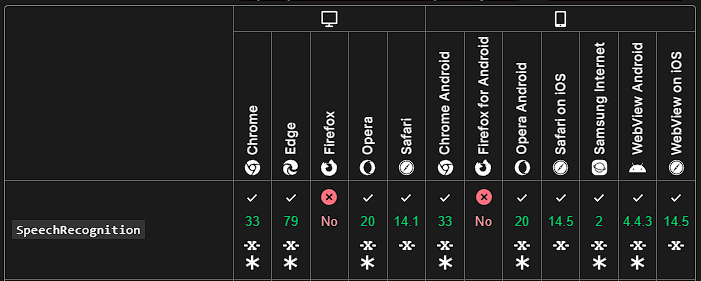
\includegraphics[width=0.8\linewidth]{img/WebSpeechAPI.png}
    \caption{Compatibilidad en exploradores}
    \label{fig:SpeechRecognitionAPI}
\end{figure}

Finalmente una de las razones por las que se opto por esta opcion es su facilidad de implementacion ya que no requiere de libreries externas, se ejecuta directamente en el navegador y es ideal para el uso de prototipos, demos o apps ligeras.

\begin{figure}[H]
    \centering
    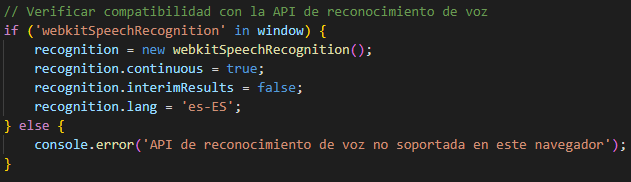
\includegraphics[width=0.8\linewidth]{img/WebKit.png}
    \caption{Ejemplo basico de WebSpeechAPI}
    \label{fig:WebKit}
\end{figure}

Como se observa en la Figura~\ref{fig:WebKit} la integración se hace en pocas líneas de código. Este codigo muestra la activacion de reconocimiento continuo \textbf{recognition.continuous = true;}, esto quiere decir que se procesara la transcripcion continuamente, pero con la condicion de devolver el resultado final gracias a \textbf{recognition.interimResults = false;} ademas de seleccionar el idioma que se desea trancribir.

Por otro lado no todo son ventajas, exites limitaciones para el uso de esta API, tales como el requerimiento de conexión a internet, ya que utiliza los servidores de Google para el reconocimiento. Ademas el soporte y el comportamiento pueden variar entre diferentes navegadores. Y sobre todo cuenta con una menor precisión en comparación con modelos como Whisper, especialmente en ambientes ruidosos o con acentos fuertes.


\subsection{AssemblyAI}

AssemblyAI\footnote{Documentacion de Assembly~\cite{assemblyai_about}.} es una plataforma de Inteligencia Artificial que ofrece potentes APIs para el procesamiento de audio, incluyendo reconocimiento de voz (Speech-to-Text), comprensión del lenguaje natural (NLP) y otras funcionalidades de inteligencia de audio.

Cuenta con caracteristicas similares al Web Speech API salvo que tiene algunas mejoras en otros puntos.

AssemblyAI se enfoca en ofrecer modelos de reconocimiento de voz de última generación entrenados en grandes cantidades de datos, lo que generalmente resulta en una mayor precisión, especialmente en entornos ruidosos o con acentos variados, con la posibilidad de identificar al hablante, detectar las emociones expresadas en el audio, incluso admite diferentes formatos de archivo y fuentes de audio/video que puedes ser en tiempo real o no.

La API es robusta y escalable, fue diseñada para desarrolladores que necesitan integrar capacidades de reconocimiento de voz en aplicaciones complejas y a gran escala. Por ello al ser una API externa, funciona de manera consistente en diferentes navegadores y plataformas, su uso en navegadores se realizara a traves de un API REST y las respuestas se reciben como respuesta a dicha API por esto requiere una conexión a internet activa para enviar y recibir datos de la API. AssemblyAI es un servicio comercial y tiene costos asociados en función del volumen de audio procesado, aunque a menudo ofrecen planes gratuitos o de prueba.

\cleardoublepage
\section{A-Frame} 
\label{sec:seccion2}

Para la implementacion en AR/VR se uso A-Frame\footnote{Véase la página de referencia de A-Frame~\cite{aframe2025}.}
, este es un framework web de codigo abierto usado para el desarollo de experiencias en realidad virtual y aumentada. Utilizando HTML como lenguaje principal para la definicion de escenas. Este framework se basa en Three.js el cual es una biblioteca de JavaScript para graficos en 3D.

A-Frame se caracteriza por el uso simplificado de Three.js para la creacion de escenas, evitando el directo y complejo gestionamiento de los detalles de renderizacion en 3D.

Usando una arquitectura llamada ECS (Entity Components System) que es aplicada a los videojuegos, en donde cada objeto es una entidad diferenciada, que puede o no albergar otras entidades. Debemos tener en cuenta que para acceder a la libreria de este framework debemos usar una linea de codigo al html que utilices \texttt{<script src="https://aframe.io/releases/1.7.0/aframe.min.js"></script>
}
esta linea de codigo utiliza para incluir la biblioteca principal de A-Frame desde un CDN (Content Delivery Network). Esta etiqueta \texttt{<script>} permite cargar la versión 1.7.0 de A-Frame directamente desde la web, dicha version puede variar.

Una de las caracteristicas mas claras de A-Frame es la definicion de entidades utilizando un etiquetado similar al de HTML. Esto per mite a desarolladores construir mundos virtuales de manera rapida y simple, como se observa en este fragmento de codigo de la Figura~\ref{lst:a-scene_Figure}: 

\begin{lstlisting}[language=HTML, caption=Escena A-Frame básica, captionpos=b,label=lst:a-scene_Figure]

      <a-scene>
        <a-box position="-1 0.5 -3" rotation="0 45 0" color="#4CC3D9"></a-box>
        <a-sphere position="0 1.25 -5" radius="1.25" color="#EF2D5E"></a-sphere>
        <a-cylinder position="1 0.75 -3" radius="0.5" height="1.5" color="#FFC65D"></a-cylinder>
        <a-plane position="0 0 -4" rotation="-90 0 0" width="4" height="4" color="#7BC8A4"></a-plane>
        <a-sky color="#ECECEC"></a-sky>
      </a-scene>
\end{lstlisting}

Cada entidad de esta escena tiene sus propiedades especificada en la pagina de la documentacion de A-Frame\footnote{Véase la documentacion de A-Frame~\cite{aframe2025docs}.}

\begin{figure}[H]
    \centering
    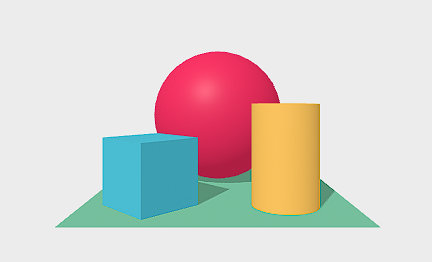
\includegraphics[width=0.5\linewidth]{img/SceneSimple.png}
    \caption{Escena simple A-Frame}
    \label{fig:aframe-scene}
\end{figure}

El núcleo de A-Frame es su sistema de entidades-componentes. Las entidades son objetos genéricos que adquieren propiedades y comportamientos mediante componentes.Los componentes son modulos reutilizables que añaden comportamientos, propiedades visuales, interacciones y varias acciones mas a las entidades. A-Frame proporciona componentes predefinidos  (como position, rotation, scale, material, geometry,\cdot. Como se puede observar en el Listado~\ref{lst:componente}, el componente \texttt{hover-color} cambia el color de la entidad al pasar el cursor sobre ella.


\begin{lstlisting}[language=HTML, caption=Crear Componente, captionpos=b, label=lst:componente]
AFRAME.registerComponent('hover-color', {
  schema: {
    color: {type: 'color', default: '#FF0000'} // color al pasar el mouse
  },
  init: function () {
    const originalColor = this.el.getAttribute('material').color;
    const newColor = this.data.color;
    this.el.addEventListener('mouseenter', () => {
      this.el.setAttribute('color', newColor);
    });
    this.el.addEventListener('mouseleave', () => {
        this.el.setAttribute('color', originalColor);
    });
  }
});
\end{lstlisting}


/****/PREGUNTAR SI HABLO DE MAS COSAS QUE SE PODRIA/****/
\cleardoublepage
\section{Three.js} 
\label{sec:seccion3}

Como mencionamos anteriormente, A-Frame se construye sobre la potente biblioteca de gráficos 3D Three.js\footnote{Learning Three.js: The 
JavaScript 3D Library for 
WebGL~\cite{dirksen2013learning}.} el cual es una biblioteca de JavaScript que facilita la creacion de graficos 3D. A-Frame abstrae la complejidad de Three.js, permitiendo a los desarrolladores centrarse en la creación de contenido sin tener que lidiar directamente con la configuración de WebGL, shaders, matrices, etc. Sin embargo, para necesidades más avanzadas, los desarrolladores pueden acceder directamente al objeto Three.js subyacente dentro de los componentes personalizados de A-Frame.
Con Three.js, puedes crear y manipular formas básicas como cubos o esferas, importar modelos complejos (en formatos como GLTF), aplicar materiales y texturas, e iluminar escenas con luces realistas. Además, incluye cámaras y controles intuitivos para navegar, así como soporte para animaciones fluidas. 

La contruccion de escenas mediante Three.js utilizara componentes como:
 
\begin{itemize}
    \item \textbf{Escena (Scene)}: el contenedor de todos los elementos 3D, como objetos, luces y cámaras.
    
    \item \textbf{Cámara (Camera)}: define el punto de vista desde el que se observa la escena. Las más comunes son la cámara de perspectiva y la ortográfica.
    
    \item \textbf{Renderizador (Renderer)}: convierte la escena y la cámara en una imagen visible en el lienzo HTML (\texttt{<canvas>}), usando WebGL.
    
    \item \textbf{Objetos (Mesh)}: representan modelos 3D, creados a partir de geometrías (formas básicas como cubos, esferas, planos, etc.) y materiales (color, textura, iluminación).
    
    \item \textbf{Luces (Light)}: iluminan la escena y permiten que los materiales reaccionen visualmente según el tipo de luz aplicada.
\end{itemize}


\cleardoublepage
\section{WebXR} 
\label{sec:seccion4}
Contextualizando este apartado debemos conocer la historia y desarollo de WebXR. Fue desarollada bajo las especificaciones del consorcio de W3C (World Wide Web)\footnote{WebXR segun W3C~\cite{w3c_webxr}.}.

Su predecesor fue WebVR

"WebVR is an open specification that makes it possible to experience immersive virtual reality in your browser."\footnote{WebVR segun W3C  ~\cite{webvr-spec}.} esta era una APÌ experimental creada unicamente para el desarollo en realidad virtual.Este standart fue algo fundamental para el desarrollo actual, pero presentaba varias limitaciones ya que no abordaba los problemas relacionados con la realidad aumentada. La evolucion y la integracion de la realidad aumentada es la que creo el actual WebXR.

WebXR(Web Extended Reality) es un conjunto de tecnologias web que permite crear experiencias en realidad virtual (VR) y en realidad aumentada (AR) dentro de navegadores. Esto implica que cualquier usuario puede acceder a estas experiencias sin necesidad de descargar aplicaciones separadas.

WebXR presenta varias funcionalidades como: 

\begin{itemize}
  
  \item \textbf{Renderizado de Escenas 3D:} Facilita el renderizado de escenas 3D en estos dispositivos a las velocidades de fotogramas adecuadas, creando la experiencia sea inmersiva.
  
  \item \textbf{Seguimiento de Movimiento:} WebXR puede rastrear el movimiento y la orientación de la cabeza y los controladores del usuario, lo que permite la interactividad.
  
  \item \textbf{Manejo de Entrada:} Admite la entrada de varios controladores y dispositivos XR, lo que permite la interacción del usuario.

\end{itemize}
Estas funcionalidades mencionadas mas otras, crean las beneficiosas caracteristicas que hacen que a este tipo de tecnologias web sean accesibles y compatibles en diferentes plataformas, aprovechando las diferentes tecnologias web familiares como JavaScript, HTML y WebGL para crear experiencias WebXR.

\cleardoublepage
\section{WebGL} 
\label{sec:seccion5}

WebGL surgio por la necesidad de llevar los graficos 3D directamente a un navegador. Antes los graficos 3D se limitaban a tecnologias basadas en plugins como "Adobe Flash" o renderizacion puramente con JavaScript, esto resultaba en una caida abrupta de rendimiento.

Creada en 2007 por el grupo Khronos\footnote{Khronos Group  ~\cite{webgl-khronos}.} fue desarollada basandose en una API conocida como OpenGL ES 2.0 diseñada para dispositivos embebidos.

"WebGL is an API that brings hardware-accelerated 3D graphics to the Web, leveraging the widely adopted OpenGL ES 2.0 standard." \cite{webgl-khronos}

Esta tecnologia fue impulsada gracias a empresas como Mozilla y Google quienes fueron actores clave para la implementacion y desarollo del WebGL.

Una de las caracteristicas mas importantes de WebGL es la capacidad de aprovechamiento de la GPU del dispositivos del usuario, permitiendo una renderizacion mas rapida y eficiente de graficos en 3D. Por otro lado la integracion en el DOM junto con otras tecnologías web como HTML, CSS y JavaScript ayudan a el desarollo de escenas en 3D. La multiplataformeidad que ofrece WebGL permite que se pueda ejecutar en cualquier navegador independientemente de su sistema operativo.
\cleardoublepage

\section{HTML} 
\label{sec:seccion6}

HTML(HyperText Markup Language) fue inventado por Tim Berners-Lee en el CERN (Organización Europea para la Investigación Nuclear) a principios de la década de 1990. Se buscaba que los cientificos pudieran compartir información fácilmente a través de una red, en donde el hipertexto de HTML\footnote{HTML W3C  ~\cite{w3c-html-intro}.} jugaba una parte esencial.

"HTML (HyperText Markup Language) is the set of markup symbols or codes inserted in a file intended for display on a World Wide Web browser page. The markup tells the Web browser how to display a Web page's words and images for the user." \cite{w3c-html-intro}   

Esta definicion de W3C muestra el proposito del HTML. A medida que la web evoluciono HTML tambien lo hizo creando diferentes versiones que se iban adaptando al uso de navegadores.

La mas moderna version el HTML5 introdujo una gran cantidad de caracteristicas, como el soporte multimedia de audio y video, ademas de la posibilidad de Canvas para graficos 2D.

El HTML como tal se conoce como lenguaje de marcado, lo que significa que utiliza etiquetas (tags) para estructurar el contenido. Estas etiquetas indican el significado y la presentación de diferentes elementos (encabezados, párrafos, imágenes, enlaces, etc.). Los documentos HTML cuentan con una estructura jerarquica basada en el anidamiento de elementos, esto permite introducir elementos o etiquetas dentro de otras, definiendo una relacion entre dichos objetos de "Padre-Hijo". HTML5 introdujo elementos semanticos como:

\begin{itemize}
  \item \texttt{<article>}: Representa un contenido independiente y autocontenido, como una publicación de blog, un artículo de noticias o una entrada en un foro.

  \item \texttt{<nav>}: Define una sección de navegación que contiene enlaces a otras partes del sitio web o a otras páginas.

  \item \texttt{<aside>}: Representa contenido relacionado pero no esencial con el contenido principal, como barras laterales, bloques de anuncios o notas.

  \item \texttt{<header>}: Define una cabecera para una sección o para toda la página. Suele incluir el título, logotipo, menú de navegación u otra información introductoria.

  \item \texttt{<footer>}: Representa el pie de página de una sección o de todo el documento. Puede contener información como derechos de autor, enlaces de contacto o créditos.

  \item \texttt{<audio>}: Permite insertar contenido de audio en una página web. Se puede usar junto con controles para reproducir, pausar o ajustar el volumen.

  \item \texttt{<video>}: Permite insertar contenido de video en la web, también con controles para reproducción, pausa y volumen, así como subtítulos o múltiples fuentes.
\end{itemize}

La mayoria de etiquetas usadas en HTML se deberan cerrar tras su uso.
\cleardoublepage
\section{JavaScript} 
\label{sec:seccion7}

"JavaScript es un lenguaje de programación interpretado que permite implementar funcionalidades complejas en páginas web, haciéndolas más dinámicas e interactivas." \cite{mdn_javascript_intro_es}

Dieñado origialmente para ejecutarse en el navegadore del cliente (front-end), hoy en dia tambien se usa en el lado del servidor (back-end) con entornos como Node.js, asi como en desarollo de aplicaciones moviles y de escritorio.

JavaScript juega un papel fundamental en el desarollo de paginas web dinamicas, dotando al HTML antes mencionado con diferentes posibilidades de accion.

Se caracteriza por la posibilidad de ser ejecutado linea a linea por el navegador, sin tener que compilarse antes de ello, ademas al ser un lenguaje de alto nivel facilita la escritura y comprension de codigo, por otro lado cuenta con un tipado de variables lo que significa que dichas "variables" pueden cambiar a lo largo de la ejecucion.

A lo largo del desarollo del proyecto se a usado en diferentes escenario, desde la creacion de un servidor simple, hasta la codificacion de componentes para A-Frame con la finalidad de dar funcionalismo a escenas en 3D desarolladas en dicho framework. Un ejemplo de ello lo tenemos presente en la Figura~\ref{fig:component-aFrame}.: 

\begin{figure}[H]
    \centering
    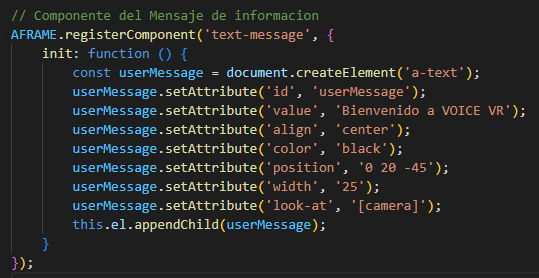
\includegraphics[width=0.8\linewidth]{img/text_msg.png}
    \caption{Creacion de un componente}
    \label{fig:component-aFrame}
\end{figure}
Este componente se usara para la iniciacion y creacion de un elemento de texto que cuenta con diferentes atributos, para luego añadirlo en la escena.

De la misma manera con JavaScript \footnote{Estructura de JavaScript~\cite{mdn_javascript_data_structures}.} jugaba una parte esencial. se pueden crear inumerables escenarios gracias a su capacidad de crean funciones de bloques de codigo que contendran acciones, objetos y/o datos que haran que las posibilidades de uso de este lenguaje de programacion sean enormes. Como por ejemplo: 

\begin{itemize}
  \item \textbf{Tipado Dinámico:} Las variables en JavaScript no están directamente ligadas a un tipo específico. Una misma variable puede contener un número, una cadena de texto y después un objeto. Esto ofrece flexibilidad pero también requiere precaución para evitar errores en tiempo de ejecución.

  \item \textbf{Tipos de Datos Primitivos:} JavaScript tiene varios tipos de datos primitivos e inmutables:
  \begin{itemize}
    \item \textbf{undefined:} Indica que una variable no tiene un valor asignado.
    \item \textbf{null:} Representa la ausencia intencional de un valor.
    \item \textbf{boolean:} Representa un valor verdadero (\texttt{true}) o falso (\texttt{false}).
    \item \textbf{number:} Representa valores numéricos (incluyendo enteros y números de punto flotante).
    \item \textbf{string:} Representa secuencias de caracteres.
    \item \textbf{bigint:} Representa enteros de longitud arbitraria.
    \item \textbf{symbol:} Representa un identificador único e inmutable.
  \end{itemize}

  \item \textbf{Objetos:} Los objetos son colecciones dinámicas de pares clave-valor. Las claves suelen ser cadenas (o símbolos), y los valores pueden ser cualquier tipo de dato, incluyendo otros objetos y funciones.

  \item \textbf{Arrays:} Los arrays son objetos especiales utilizados para almacenar colecciones ordenadas de elementos. Pueden contener elementos de diferentes tipos.

  \item \textbf{Funciones:} Bloques de código reutilizables que pueden recibir argumentos y devolver valores. Pueden ser tratadas como cualquier otro valor.

  \item \textbf{Asincronía:} JavaScript es fundamentalmente asíncrono para manejar operaciones que pueden llevar tiempo (como peticiones de red o manipulación del DOM) sin bloquear el hilo principal.
  
  \item \textbf{Promesas:} Las \textit{Promesas} (\texttt{Promise}) son objetos que representan el resultado eventual (éxito o fallo) de una operación asíncrona, facilitando el manejo de código asíncrono. \texttt{async/await} es una sintaxis más moderna y legible construida sobre las Promesas.
  
\end{itemize}

\cleardoublepage
\section{CSS} 
\label{sec:seccion8}
CSS (Cascading Style Sheets) es como la cobertura y la decoración de una página web (el HTML seria el esqueleto). Se usa para decirle al navegador cómo mostrar los elementos de HTML: qué colores usar, qué fuentes, cómo se deben organizar en la pantalla, si deben tener márgenes, bordes, etc. Existen tres formas principales de usar CSS:

\begin{itemize}
  \item En la misma línea (\texttt{Inline}): Se aplica directamente a elementos HTML individuales usando el atributo style. No es la forma recomendada para la mayoría de los casos porque dificulta mucho mantener la consistencia y el orden como se ve en la Figura~\ref{fig:Style_line}.
\begin{figure}[H]
    \centering
    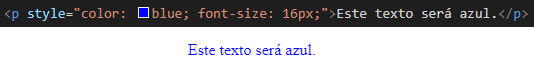
\includegraphics[width=0.8\linewidth]{img/style1.png}
    \caption{Primera forma de usar CSS}
    \label{fig:Style_line}
\end{figure}

\item En el encabezado (\texttt{Internal}): Se coloca dentro de la sección \texttt{<head>} de un documento HTML, entre etiquetas \texttt{<style>}. Es útil para estilos específicos de una sola página como se ve en la Figura~\ref{fig:Style_Internal}.
\begin{figure}[H]
    \centering
    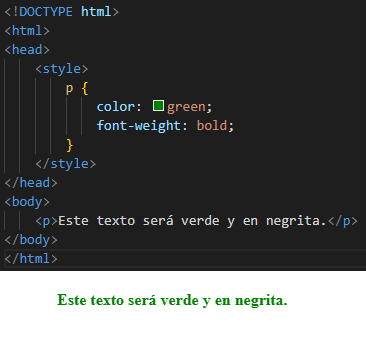
\includegraphics[width=0.6\linewidth]{img/Style2.png}
    \caption{Segunda forma de usar CSS}
    \label{fig:Style_Internal}
\end{figure}

\item En un archivo separado (\texttt{External}): Esta es la forma más común y recomendada. Se crea un archivo con extensión .css (por ejemplo, estilos.css) y se vincula al documento HTML usando la etiqueta \texttt{<link>} dentro de la sección \texttt{<head>}.como se ve en la Figura~\ref{fig:Style_External}.
\begin{figure}[H]
    \centering
    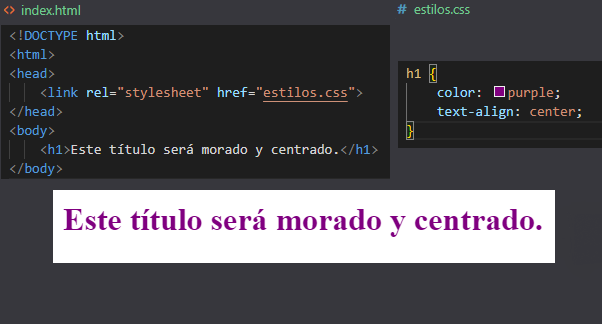
\includegraphics[width=0.8\linewidth]{img/Style3.png}
    \caption{Tercera forma de usar CSS}
    \label{fig:Style_External}
\end{figure}


\end{itemize}
\cleardoublepage

\section{NodeJS} 
\label{sec:seccion9}

Node.js es un entorno de ejecución de JavaScript de código abierto y multiplataforma. Permite ejecutar código JavaScript fuera de un navegador web.

Node.js fue creado por Ryan Dahl y se lanzó inicialmente en 2009. Se estaba buscando una forma más eficiente de manejar conexiones y concurrencia en la web después de experimentar problemas con el servidor web Apache. Se inspiró en lenguajes orientados a eventos y propuso una arquitectura basada en un bucle de eventos no bloqueante, La clave de esto fue la utilizacion del motor V8 presente en google Chrome, el cual compilada JavaScript de manera rapida y eficiente.

Node.js se centra en una arquitectura orientada a eventos y no bloqueante, esto significa que en lugar de esperar a que una operación de entrada/salida (E/S) se complete (bloqueando el hilo), Node.js registra una función de callback que se ejecutará una vez que la operación finalice. Esto permite manejar muchas conexiones simultáneas de manera eficiente con un solo hilo. 

Existen problemas con lo anterior mencionado, uno de los mas importantes era el anidamiento de callback ya que con un numero excesivamente grande de estos, la lectura y mantencion de estas de vuelve dificil. Este problema se mitigo con la llegada de las promesas y las funciones \texttt{async/await}. Tambien el uso de tareas complejas podrian sobrecargar la CPU y afectar negativamente al hilo principal. 

\subsection{Node.js y el Manejo de Peticiones HTTP} 

Node.js es excelente para manejar peticiones HTTP, tanto para crear servidores web que responden a las solicitudes de los clientes (navegadores, otras aplicaciones) como para realizar peticiones a otros servidores (APIs externas).

\begin{itemize}
  \item \textbf{Módulo \texttt{http} y \texttt{https}:} Node.js proporciona módulos nativos (\texttt{http} para HTTP y \texttt{https} para HTTPS) para crear servidores y clientes HTTP/HTTPS de bajo nivel.

  \item \textbf{Frameworks (Express, Koa):} Frameworks como \texttt{Express} simplifican enormemente la creación de servidores web, proporcionando funcionalidades para el enrutamiento, el manejo de middleware, la gestión de solicitudes y respuestas, etc.

  \item \textbf{Clientes HTTP:} Para realizar peticiones a otros servidores, se pueden usar los módulos nativos (\texttt{http}, \texttt{https}) o bibliotecas de terceros más convenientes como \texttt{axios} o \texttt{node-fetch}.

  \item \textbf{Manejo de Métodos HTTP:} Node.js facilita el manejo de diferentes métodos HTTP (\texttt{GET}, \texttt{POST}, \texttt{PUT}, \texttt{DELETE}, etc.) para construir APIs RESTful.

  \item \textbf{Streams:} Node.js utiliza \textit{streams} para manejar grandes cantidades de datos de manera eficiente durante las peticiones y respuestas, evitando cargar todo en la memoria.
\end{itemize}
\subsection{Certificados} 

Para asegurar las comunicaciones a través de la web (HTTPS), Node.js permite trabajar con certificados SSL/TLS:

\begin{itemize}
  \item \textbf{Módulo \texttt{https}:} El módulo \texttt{https} permite crear servidores HTTPS configurando las opciones del certificado (clave privada, certificado, certificados de autoridad \textit{CA} si es necesario).

  \item \textbf{Obtención de Certificados:} Los certificados se pueden obtener de autoridades de certificación (CA) como \textit{Let's Encrypt} (que ofrece certificados gratuitos) o de proveedores comerciales. También se pueden generar certificados auto-firmados para entornos de desarrollo o pruebas (aunque no son confiables para producción).

  \item \textbf{Configuración del Servidor:} Al crear un servidor HTTPS en Node.js, se deben especificar las rutas a los archivos del certificado y la clave privada en las opciones de configuración.

  \item \textbf{Manejo de Peticiones Seguras:} Una vez configurado el servidor HTTPS, Node.js manejará automáticamente el cifrado y descifrado de las comunicaciones.

  \item \textbf{Clientes HTTPS:} Al realizar peticiones HTTPS a otros servidores, Node.js (a través del módulo \texttt{https} o bibliotecas como \texttt{axios}) maneja la verificación del certificado del servidor remoto (si está configurado correctamente con una CA de confianza).
\end{itemize}

\cleardoublepage
\section{Aplicaciones con reconocimiento de Voz} 
\label{sec:seccion10}
El reconocimiento de voz está abriendo muchas posibilidades interesantes en diversas aplicaciones y juegos, incluyendo experiencias en gafas de realidad virtual (VR) y realidad aumentada (AR). Aquí te presento algunos ejemplos:

\subsection{Arkio:}

Arkio es una herramienta de diseño espacial colaborativo que permite a las personas crear y colaborar utilizando Realidad Virtual (VR), así como en PC, tablet y móvil.

\begin{itemize}
  \item Se centra en el diseño de interiores, edificios, espacios virtuales y planificación urbana.
  
  \item No se menciona explícitamente el control por voz como una característica principal en las descripciones disponibles. La interacción parece basarse principalmente en los controladores VR y las interfaces en las otras plataformas.
  
  \item Permite el modelado sólido rápido con operaciones booleanas y volúmenes paramétricos.
  
  \item Facilita la colaboración multiplataforma en tiempo real.
  
  \item Dispone de plugins para integrar con herramientas de diseño 3D como \texttt{Revit}, \texttt{Rhino} y \texttt{SketchUp}, permitiendo importar modelos existentes y exportar el trabajo realizado en Arkio.
  
  \item Arkio permite a los usuarios dibujar y manipular elementos arquitectónicos de forma intuitiva en el espacio VR.
\end{itemize}

\subsection{VR Sculpting:}
VR Sculpting con Comandos de Voz: En la escultura VR (como en Oculus Medium o Gravity Sketch), se han explorado o implementado (a menudo a través de plugins o herramientas de terceros como VoiceAttack) comandos de voz para tareas específicas durante el proceso de modelado. Por ejemplo, podrías usar la voz para:
\begin{itemize}
    \item Seleccionar herramientas: "Seleccionar herramienta de arcilla", "Cambiar a herramienta de suavizado".
    \item Modificar parámetros: "Aumentar tamaño del pincel", "Reducir intensidad".
    \item Realizar acciones: "Crear esfera", "Extruir esta superficie", "Duplicar objeto".
\end{itemize}
Si bien esto no es la creación del objeto desde cero con la voz, sí permite una manipulación y modificación significativa mediante comandos hablados.
***** DESAROLLAR MAS

\subsection{Bridge Crew:}
Bridge Crew (Star Trek): Permite dar órdenes verbales a la tripulación, lo que implica una interacción por voz para controlar elementos del juego.

***** DESAROLLAR MAS
//// BUSCAR OTRAS APLICACIONES DE CREADORES DE OBJETOS EN VR CON VOZ O LOS QUE CREAN ESCENAS SIN NECESIDAD DE VOZ
JUEGOS TAMBIEN cuentan ** por si acaso que sea de voz 

\cleardoublepage

\chapter{Desarrollo del proyecto}
\label{chap:Desarollo}
 A este proceso se aplicó estrategias basadas en metodologías ágiles Scrum para organizar el trabajo, un marco que facilita la gestión de proyectos complejos mediante ciclos iterativos conocidos como sprints.  Hasta que no se consigue el objetivo de un sprint no comienza el otro, y la consecución de los objetivos de todos los sprints coincide con la consecución del objetivo final del proyecto. Estos sprints a su vez se dividen en tareas mucho más pequeñas que persiguen objetivos más concretos y ayudan a la consecución del objetivo final del sprint.

Estructura mínima de cada sprint:
\begin{itemize}
\item Especificación
\item Tareas
\item Prototipo resultado
\item Lecciones aprendidas
\end{itemize}

\section{Arquitectura general} 
\label{sec:arquitectura}


\begin{figure}[H]
  \centering
  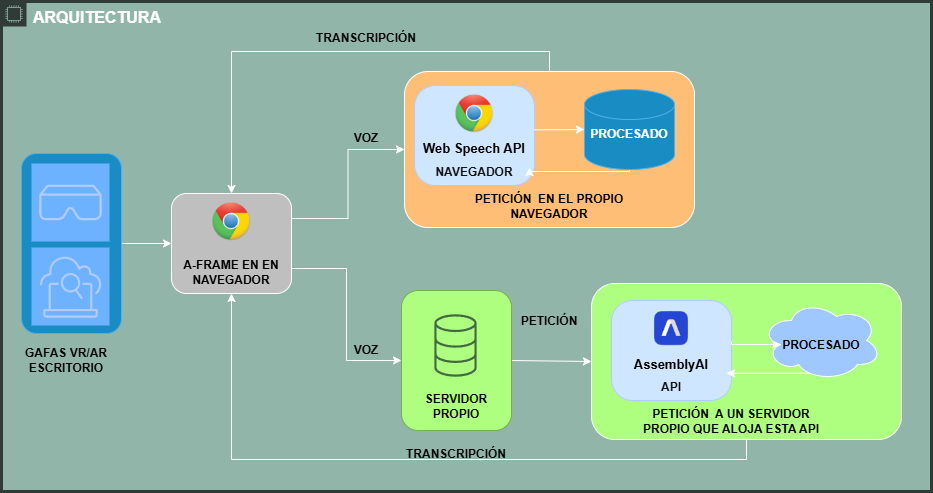
\includegraphics[width=14cm, keepaspectratio]{img/Arquitectura.png}
  \caption{Estructura del funcionamiento del Proyecto}
  \label{fig:arquitectura}
\end{figure}


El diagrama de la Figura~\ref{fig:arquitectura} muestra dos arquitecturas distintas para transcribir voz en una aplicación web VR/AR construida con A-Frame. En la primera demo, la transcripción se realiza directamente en el navegador usando la Web Speech API. Esto permite capturar la voz y procesarla sin necesidad de servidores externos, lo cual es rápido pero depende del soporte del navegador. En la segunda demo, la voz se envía a un servidor propio, que luego la reenvía a la API de AssemblyAI para su transcripción. Esta opción ofrece mayor precisión y capacidades avanzadas, aunque requiere una infraestructura adicional y puede tener más latencia.



%%%%%%%%%%%%%%%%%%%%%%%%%%%%%%%%%%%%%%%%%%%%%%%%%%%%%%%%%%%%%%%%%%%%%%%%%%%%%%%%
%%%%%%%%%%%%%%%%%%%%%%%%%%%%%%%%%%%%%%%%%%%%%%%%%%%%%%%%%%%%%%%%%%%%%%%%%%%%%%%%
% EXPERIMENTOS Y VALIDACIÓN %
%%%%%%%%%%%%%%%%%%%%%%%%%%%%%%%%%%%%%%%%%%%%%%%%%%%%%%%%%%%%%%%%%%%%%%%%%%%%%%%%

\cleardoublepage

\begin{itemize}
\item Sprint 1: Investigacion sobre uso, posible desarollo y funcion de los objetos relacionados al proyecto.
\item Sprint 2: Desarollo e investigacion de reconocimiento de voz.
\item Sprint 3: Desarollo de la primera demo sobre funcionamiento de A-FRAME.
\item Sprint 4: Creacion de objetos de A-FRAME simples.
\item Sprint 5: Creacion de componentes para A-FRAME y reestructuracion de codigo.
\item Sprint 6: Creacion de funcionalidades para componentes.
\item Sprint 7: Intento de integracion con gafas VR/AR
\item Sprint 8: Aumento de comandos para la funcionalidad del proyecto.
\item Sprint 9: Creacion de servidor propio para Peticiones de Transcripcion
\item Sprint 10: Creacion de escena simple para funcionalidad en escritorio
\item Sprint 11: Mejora de la estetica y colocacion de objetos.
\item Sprint 12: Implementacion de plugins extra para la visualizacion y decoraciones.
\end{itemize}

\section{Sprint 1} 
\label{sec:sprint1}
\subsection{Whisper}
Durante este Sprint se llevo a cabo la 


%%% APARTIR DE AQUI LOS SPRINTS NECESITAN MAS DESAROLLO, DEJO COMENTADOS UNOS DATOS A COMPLETAR.
\section{Sprint 2} 
\label{sec:sprint2}

Se desarrollaron **tres ejemplos** para demostrar cómo implementar reconocimiento de voz en distintos contextos:
\subsection{Objetivos}

- Explorar y comparar distintas tecnologías de reconocimiento de voz.
- Evaluar precisión, facilidad de implementación y rendimiento.
- Servir como base para futuros desarrollos más avanzados.

\subsection{Programa en Python (Reconocimiento con Whisper)}

- Utiliza el modelo **Whisper** de OpenAI para transcripción de audio.

- Permite convertir archivos de audio a texto con alta precisión.

- Ideal para pruebas locales y procesamiento por lotes.

- Compatible con múltiples idiomas y resistente a ruido de fondo.

\subsection{Programa en Node.js + Python (Servidor backend híbrido)}

- El servidor está hecho en **Node.js** con `Express`.

- Recibe archivos de audio desde el cliente.

- Llama internamente a un **script en Python** que utiliza **Whisper** para realizar la transcripción.

- Devuelve el texto transcrito al cliente.

- Combina lo mejor de ambos mundos: la flexibilidad de Node y la potencia de Whisper.

- No llego a funcionar por que necesitaba permisos.

\subsection{Programa para Navegador (Reconocimiento en el cliente)}

- Basado en la **Web Speech API** del navegador.

- Captura y transcribe voz directamente desde el navegador, en tiempo real.

- No requiere backend ni dependencias externas.


\section{Sprint 3} 
\label{sec:sprint3}

En este Sprint se planteo el primer contacto con el framework haciendo dos demos sencillas en las que se dara uso a un \textbf{<a-text>}.
\subsection{Objetivos}
\begin{itemize}
    \item comenzar a experimentar con la integración de **texto dinámico** en escenas 3D
    \item vincularlo con **reconocimiento de voz**, para mostrar contenido en tiempo real dentro del entorno virtual.
\end{itemize}

\subsection{Demo 1 – Texto Dinámico con A-Frame} 

- Se crea una escena con un plano (`a-plane`) y un texto (`a-text`) posicionado sobre él.
- El contenido del texto se puede modificar escribiendo desde un campo de entrada HTML o desde el código.
- Esta demo demuestra cómo manipular dinámicamente elementos de A-Frame desde JavaScript estándar.
  


\subsection{Demo 2 – Reconocimiento de Voz + A-Frame}

- Extiende la demo anterior agregando reconocimiento de voz desde el navegador (usando `Web Speech API`).
- Al hablar, el texto reconocido aparece automáticamente en el elemento `a-text` dentro de la escena.
- La experiencia permite mostrar mensajes de voz directamente dentro de un entorno 3D.  

**Cómo funciona:**

1. El usuario activa el reconocimiento de voz o de texto(por botón o al entrar a la escena).
2. El navegador convierte la voz en texto o el texto escrito.
3. El texto se muestra en tiempo real dentro del plano de A-Frame en un \textbf{<a-text>}.


\section{Sprint 4} 
\label{sec:sprint4}
Creacion de objetos de A-FRAME simples.
\section{Sprint 5} 
\label{sec:sprint5}
Creacion de componentes para A-FRAME y reestructuracion de codigo.
\section{Sprint 6} 
\label{sec:sprint6}
Creacion de funcionalidades para componentes.

\chapter{Descripción del resultado}
\label{chap:descripcion}

se necesita el uso del "NOMBRE DEL-.js" para el uso en html con la llamada a el scrpit y poner el componente en una entidad de la scena...
ademas de un componente que almacene los objetos llamado "xxx"

** SEGUIR CON ESTO **

Descripción para usuario (manual de usuario)
Descripción de la implementación


\chapter{Experimentos y validación}
\label{chap:experimentos}

** AÑADIR IMAGENES, RESULTADOS Y OPINIONES DE LOS USUARIOS **

Pequeños experimentos que muestren que se cumplen los objetivos
Si es una aplicación con interfaz de usuario, donde lo fundamental es la interacción con el usuario, realizar algún experimento con usuarios, si es posible distintos del autor del TFG.

Este capítulo se introdujo como requisito en 2019. 
Describe los experimentos y casos de test que tuviste que implementar para validar tus resultados. 
Incluye también los resultados de validación que permiten afirmar que tus resultados son correctos. 


%%%%%%%%%%%%%%%%%%%%%%%%%%%%%%%%%%%%%%%%%%%%%%%%%%%%%%%%%%%%%%%%%%%%%%%%%%%%%%%%
%%%%%%%%%%%%%%%%%%%%%%%%%%%%%%%%%%%%%%%%%%%%%%%%%%%%%%%%%%%%%%%%%%%%%%%%%%%%%%%%
% RESULTADOS %
%%%%%%%%%%%%%%%%%%%%%%%%%%%%%%%%%%%%%%%%%%%%%%%%%%%%%%%%%%%%%%%%%%%%%%%%%%%%%%%%

\cleardoublepage
\chapter{Resultados}
\label{chap:resultados}

MEDICIONES DE TIEMPO PARA LAS RESPUESTAS, Y LOS CAMBIOS EN LA ESCENA ....


%%%%%%%%%%%%%%%%%%%%%%%%%%%%%%%%%%%%%%%%%%%%%%%%%%%%%%%%%%%%%%%%%%%%%%%%%%%%%%%%
%%%%%%%%%%%%%%%%%%%%%%%%%%%%%%%%%%%%%%%%%%%%%%%%%%%%%%%%%%%%%%%%%%%%%%%%%%%%%%%%
% CONCLUSIONES %
%%%%%%%%%%%%%%%%%%%%%%%%%%%%%%%%%%%%%%%%%%%%%%%%%%%%%%%%%%%%%%%%%%%%%%%%%%%%%%%%

\cleardoublepage
\chapter{Conclusiones}
\label{chap:conclusiones}


\section{Consecución de objetivos}
\label{sec:consecucion-objetivos}

Esta sección es la sección espejo de las dos primeras del capítulo de objetivos, donde se planteaba el objetivo general y se elaboraban los específicos.

Es aquí donde hay que debatir qué se ha conseguido y qué no. 
Cuando algo no se ha conseguido, se ha de justificar, en términos de qué problemas se han encontrado y qué medidas se han tomado para mitigar esos problemas.

Y si has llegado hasta aquí, siempre es bueno pasarle el corrector ortográfico, que las erratas quedan fatal en la memoria final.
Para eso, en Linux tenemos aspell, que se ejecuta de la siguiente manera desde la línea de \emph{shell}:

\begin{verbatim}
  aspell --lang=es_ES -c memoria.tex
\end{verbatim}


\section{Esfuerzo y recursos dedicados}
\label{sec:esfuerzo-recursos}

Si es posible, con una descripción temporal (tantas horas durante tal periodo, etc) por sprint
Estimación total
Incluir el tiempo de aprendizaje
Incluir el tiempo de preparación de la memoria

Para eso, en Linux tenemos aspell, que se ejecuta de la siguiente manera desde la línea de \emph{shell}:

\subsection{Planificación temporal}
\label{sec:planificacion-temporal}

A mí me gusta que aquí pongáis una descripción de lo que os ha llevado realizar el trabajo.
Hay gente que añade un diagrama de GANTT.
Lo importante es que quede claro cuánto tiempo llevas (tiempo natural, p.ej., 6 meses) y a qué nivel de esfuerzo (p.ej., principalmente los fines de semana).

\begin{verbatim}
  aspell --lang=es_ES -c memoria.tex
\end{verbatim}


\section{Aplicación de lo aprendido}
\label{sec:aplicacion}
sobre impacto de asignaturas de la carrera, tanto concimientos útiles, como cosas que ha habido que aprender que no se han enseñado en la carrera
****


Aquí viene lo que has aprendido durante el Grado/Máster y que has aplicado en el TFG/TFM.
Una buena idea es poner las asignaturas más relacionadas y comentar en un párrafo los conocimientos y habilidades puestos en práctica.

\begin{enumerate}
  \item a
  \item b
\end{enumerate}


\section{Lecciones aprendidas}
\label{sec:lecciones_aprendidas}

Aquí viene lo que has aprendido en el Trabajo Fin de Grado/Máster.

\begin{enumerate}
  \item Aquí viene uno.
  \item Aquí viene otro.
\end{enumerate}


\section{Trabajos futuros}
\label{sec:trabajos_futuros}

Ningún proyecto ni software se termina, así que aquí vienen ideas y funcionalidades que estaría bien tener implementadas en el futuro.

Es un apartado que sirve para dar ideas de cara a futuros TFGs/TFMs.


%%%%%%%%%%%%%%%%%%%%%%%%%%%%%%%%%%%%%%%%%%%%%%%%%%%%%%%%%%%%%%%%%%%%%%%%%%%%%%%%
%%%%%%%%%%%%%%%%%%%%%%%%%%%%%%%%%%%%%%%%%%%%%%%%%%%%%%%%%%%%%%%%%%%%%%%%%%%%%%%%
% APÉNDICE(S) %
%%%%%%%%%%%%%%%%%%%%%%%%%%%%%%%%%%%%%%%%%%%%%%%%%%%%%%%%%%%%%%%%%%%%%%%%%%%%%%%%

\cleardoublepage
\appendix
\chapter{Manual de usuario}
\label{app:manual}

Esto es un apéndice.
Si has creado una aplicación, siempre viene bien tener un manual de usuario.
Pues ponlo aquí.

%%%%%%%%%%%%%%%%%%%%%%%%%%%%%%%%%%%%%%%%%%%%%%%%%%%%%%%%%%%%%%%%%%%%%%%%%%%%%%%%
%%%%%%%%%%%%%%%%%%%%%%%%%%%%%%%%%%%%%%%%%%%%%%%%%%%%%%%%%%%%%%%%%%%%%%%%%%%%%%%%
% BIBLIOGRAFIA %
%%%%%%%%%%%%%%%%%%%%%%%%%%%%%%%%%%%%%%%%%%%%%%%%%%%%%%%%%%%%%%%%%%%%%%%%%%%%%%%%

\cleardoublepage

% Las siguientes dos instrucciones es todo lo que necesitas
% para incluir las citas en la memoria
\bibliographystyle{abbrv}
\bibliography{memoria}  % memoria.bib es el nombre del fichero que contiene
% las referencias bibliográficas. Abre ese fichero y mira el formato que tiene,
% que se conoce como BibTeX. Hay muchos sitios que exportan referencias en
% formato BibTeX. Prueba a buscar en http://scholar.google.com por referencias
% y verás que lo puedes hacer de manera sencilla.
% Más información: 
% http://texblog.org/2014/04/22/using-google-scholar-to-download-bibtex-citations/

\end{document}
